\documentclass{article}
\usepackage[utf8]{inputenc}
\title{MATH 20C Notes - Week Four}
\author{C-Rin}
\date{October 2019}

\usepackage{natbib}
\usepackage{graphicx}
\usepackage{gensymb}
\usepackage{amsmath}
\usepackage{amssymb}

\usepackage{diffcoeff}


\graphicspath{ {./images/} }

\begin{document}

\maketitle

\section*{Introduction}
Deep 

\begin{figure}[h!]
\centering
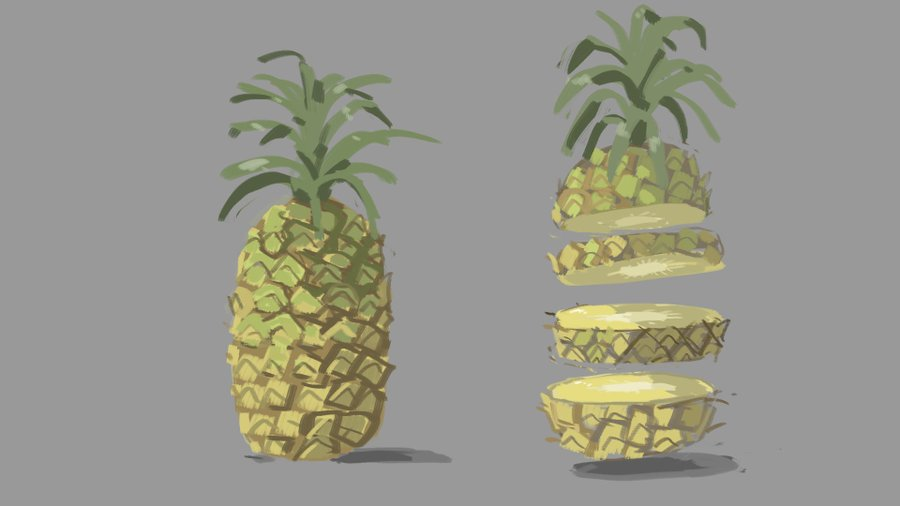
\includegraphics[scale=0.25]{pineapple.jpg}
\caption{A pineapple and a cross section of a pineapple}
\end{figure}


\newpage
\section{Paths and Curves}
\[\bar{f}:\mathbb{R} \rightarrow\mathbb{R}^n\]
If the domain of \textit{f} is the real numbers of some interval $[a,b]$, we say \textit{f} is a \underline{path}

The range is called a curve.

\subsection*{Example}
The parameterization of a line $\bar{f}(t)=(1,1,0)+t(2,1,1)$
\begin{figure}[h!]
    \centering
    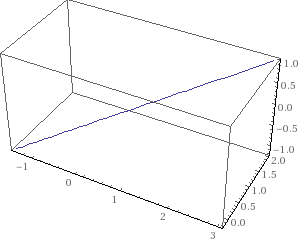
\includegraphics[scale=0.5]{images/parametric.png}
    \caption{The range is the line}
    \label{}
\end{figure}

\subsection*{Example}
\[\bar{f}(t): [0,2\pi]\rightarrow\mathbb{R}\]
\[t\rightarrow\bar{f}(t)=(\cos (t),\sin (t))\]
\begin{figure}[h!]
    \centering
    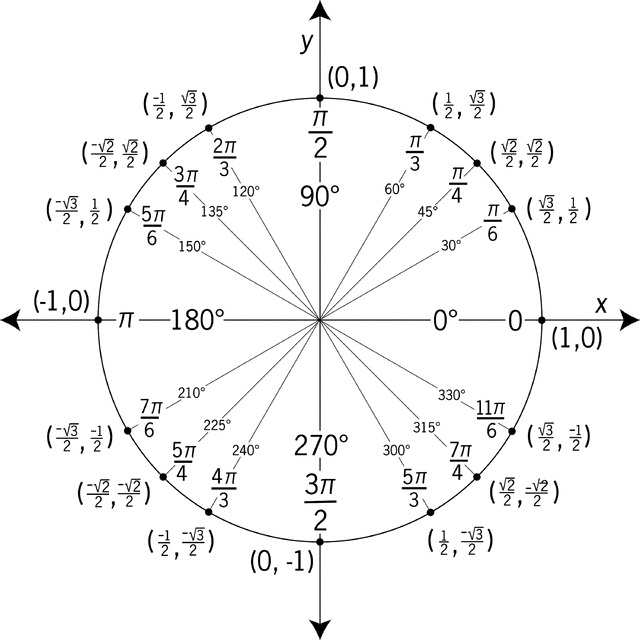
\includegraphics[scale=0.25]{unitCircle.jpg}
    \caption{Curve is the Unit Circle}
    \label{}
\end{figure}

\subsection*{Example: Wheel with Ant}
In this example, we have wheel moving at $1 m/s$ with a radius of $1$ meter, and an ant on the perimeter of the wheel. 
We want to parameterize the ant's position at time \textit{t}.\\[6pt]
Let ant(t) denote the location of the ant.\\
The location of the center is $(0,1) \mbox{ at }t=0 $, and the location of the center is $(t,1)$\\
At the time \textit{t}, we need the angle of the ant $\theta(t)$

\[\mbox{Starting angle}=\frac{-\pi}{2}\]
\[\mbox{At angle $\theta$, the wheel has traveled }\theta=t\]
\[\theta_{ant}(t)=-\frac{\pi}{2}-t\]
\[ant(t)=(t,1)+(\cos(\frac{-\pi}{2}-t),\sin(\frac{-\pi}{2}-t))\]

Given a path $\bar{f}(t):\mathbb{R}\rightarrow\mathbb{R}^3$\\[6pt]
The \underline{velocity} of the path at time$(t)$ is $D\bar{f}(t)$\\[6pt]
The speed of the path at time \textit{t} is $||D\bar{f}(t)||$\\[6pt]
The velocity is the direction of the tangent line of the path
If velocity $\neq$ 0, then the velocity points in the direction of the curve.
\begin{figure}[h!]
    \centering
    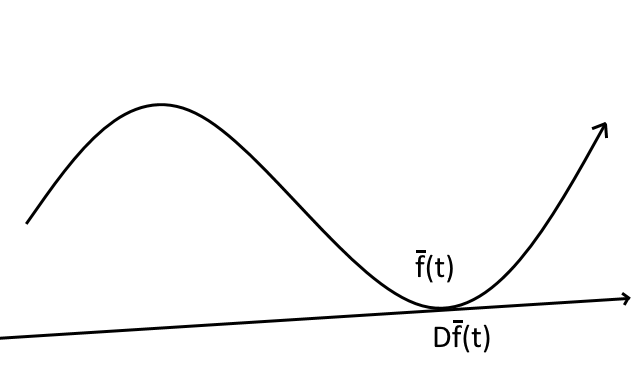
\includegraphics[scale =.5]{line.png}
    \caption{Can parameterize \textit{l}}
    \label{}
\end{figure}
The tangent line of time $t_o$ is parameterized by $l(t)==f(t_o)+t\cdot(D\bar{f}(t_o))$
\newpage
\subsection*{Example: The Unit Circle}
\[\bar{f}(t)=(t,\cos(t),\sin(t))\]
\begin{figure}[h!]
    \centering
    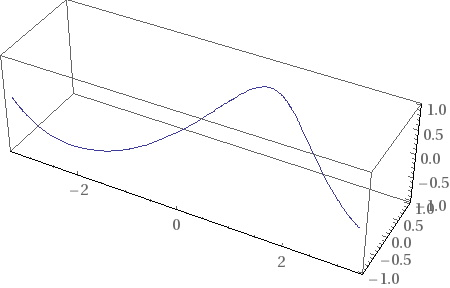
\includegraphics[scale=.5]{spiral.jpg}
    \caption{The Spiral}
    \label{}
\end{figure}
\newpage
We want to find the equation for the tangent line at $t=0$.To do this, we need to find the direction (i.e. $D\bar{f}(0)$).

\[D\bar{f}(0)=\begin{bmatrix}
    x(0)\\
    y(0)\\
    z(0)
\end{bmatrix}=\begin{bmatrix}
    1\\
    -\sin(t)\\
    cos(t)
\end{bmatrix}=\overbrace{\begin{bmatrix}
    1\\
    0\\
    1
\end{bmatrix}}^{\begin{subarray}
    \mbox{Think of this}\\
    \mbox{like a row vector}
\end{subarray}}\]

\[l(t)=(0,1,0)+t(1,0,1)\]

\subsection*{Exercise}
Find the speed of the path $(t,t^2,e^t)$ at time 0.

\[\bar{f}(0)=(0,0,1)\]
\[D\bar{f}(0)=\begin{bmatrix}
    1\\
    2t\\
    e^t
\end{bmatrix}=\begin{bmatrix}
    1\\
    0\\
    1
\end{bmatrix}\]
\[||D\bar{f}(0)=||(1,0,1)||=\sqrt{1^2+0^2+1^2}=\sqrt{2}\]
\[l(t)=(0,0,1)+t(1,0,1)\]

\section{Properties of the Derivative}
\[\overbrace{\bar{f}:\mathbb{R}^m\rightarrow\mathbb{R}^n}^{\mbox{The derivative of $D\bar{f}$ is an }\overbrace{n}^{\begin{subarray}
    \mbox{n}\\
    \mbox{row}
\end{subarray}}\times\overbrace{m}^{\begin{subarray}
    \mbox{m}\\
    \mbox{columns}
\end{subarray}}\mbox{matrix}} \]

\subsection*{Theorem}
\begin{enumerate}
    \item If c is a real number (constant)
    \begin{itemize}
        \item $Dc\bar{f}(\vec{v})=c\cdot D\bar{f}(\vec{v})$
        \item Every entry in the matrix is multiplied by c
    \end{itemize}
    \item Suppose $g:\mathbb{R}^m\rightarrow\mathbb{R}^n$
    \begin{itemize}
        \item $D(\bar{f}+\bar{g})(\vec{v})=(D\bar{f}(\vec{v}))+(D\bar{f}(\vec{v}))$
        \item Add each component individually based on their coordinate
    \end{itemize}
    \item (Product Rule) Suppose $f:\mathbb{R}^n\rightarrow\mathbb{R}$ and $g: \mathbb{R}^n\rightarrow\mathbb{R}$ are two scalar functions
    \begin{itemize}
        \item $D(f\circ g)(\vec{v})=f(\vec{v})\cdot Dg(\vec{v})+g(\vec{v}\cdot Df(\vec{v}))$
    \end{itemize}
    \item (Quotient Rule) 
    \begin{itemize}
        \item $D(\frac{f}{g})(\vec{v})=\frac{g(\vec{v})\cdot Df(\vec{v})-f(\vec{v}\cdot Dg(\vec{v}))}{(g\vec{v})^2}$
    \end{itemize}
\end{enumerate}

\subsection*{Example}
\[h:\mathbb{R}^3\rightarrow\mathbb{R}\]
\[h(x,y,z)=\frac{x^2+y^2}{z^2+1}\]
\[Dh(x,y,z)=\frac{(z^2+1)D(x^2+y^2)-(x^2+y^2)D(z^2+1)}{(z^2+1)^2}\]
\[=\frac{(z^2+1)\cdot (2x,2y,0)-(x^2+y^2)\cdot (0,0,2z)}{(z^2+1)^2}\]
\[=(\frac{2x}{z^2+1},\frac{2y}{z^2+1},\frac{-(x^2+y^2)(2z)}{(z^2+1)^2})\]
\subsection*{Exercise}
$f(x,y,z)=\sin(xy)\cos(yz)$\\
Compute $\nabla f(x,y,z)$
\[f(x,y,z)=\sin(xy)\cos(yz)\]
\[Df(x,y,z)=\sin(xy)\cdot D\cos(yz)+\cos(yz)\cdot D\sin(xy)\]
\[=\sin(xy)(0,-z\sin(yz),-y\sin(yz)+\cos(yz)\cdot(y\cos(xy),x\cos(xy),0)\]
\[=(y\cos(yz)\cos(xy),x\cos(xy)\cos(yz)-z\sin(xy)\sin(yz),-y\sin(xy)\sin(yz))\]


\section{Chain Rule}
The derivative of composed functions is a Product
\[f:\mathbb{R}^n\rightarrow\mathbb{R}^k\mbox{     }g:\mathbb{R}^k\rightarrow\mathbb{R}^m\]

\subsection{Matrix Multiplication}
\[A= \overbrace{\begin{bmatrix}
    1&2\\
    3&4
\end{bmatrix}}^{\mbox{2x2}}\qquadB=\overbrace{\begin{bmatrix}
    0&1&2\\
    3&4&0
\end{bmatrix}}^{\mbox{2x3}}\]
\[2\times [2] \overbrace{\longleftrightarrow}^{\begin{subarray}
    \mbox{Needs}\\
    \mbox{to be}\\
    \mbox{the same}
\end{subarray}} [2]\times 3\]

\begin{center}
    $A\cdot B = $
    \begin{tabular}{lll}
        \hline
        $(1,2)\cdot (0,3)$ & $(1,2)\cdot (1,4)$ & $(1,2)\cdot (2,0)$ \\ \hline
        $(3,4)\cdot (0,3)$ & $(3,4)\cdot (1,4)$ & $(3,4)\cdot (2,0)$ \\ \hline
    \end{tabular}
    $=\begin{bmatrix}
        6&9&2\\
        12&19&6
    \end{bmatrix}$
\end{center}

\[A = m\times k\qquad B=k\times n\]
\mbox{}
\[\overbrace{A\cdot B}^{\mbox{m $\times$ n matrix}}=\begin{bmatrix}
    row(1,A)\cdot column(1,B)& \ldots&row(1,A)\cdot column(j,B)\\
    \vdots&\ddots&\vdots\\
    row(i,A)&\ldots&row(i,A)\cdot column(j,B)
\end{bmatrix}\]
\subsection*{Exercise}
\textbf{1)} 
\[A\cdot B\]
\[A=\begin{bmatrix}
    1&2&4&6
\end{bmatrix}\qquadB=\begin{bmatrix}
    1\\
    1\\
    1\\
    1
\end{bmatrix}\]

\[\overbrace{A\cdot B}^{\mbox{1 $\times$ 1 }}=[13]\]


\textbf{2)}
\[C\cdot D\]
\[C=\begin{bmatrix}
    1&1\\
    1&2
\end{bmatrix}\qquadD=\begin{bmatrix}
    0&1\\
    1&0
\end{bmatrix}\]

\[C\cdot D=\begin{bmatrix}
    (1,1)\cdot (0,1)&(1,1)\cdot (1,0)\\
    (1,2)\cdot (0,1)&(1,2)\cdot (1,0)
\end{bmatrix}=\begin{bmatrix}
    1&1\\
    2&1
\end{bmatrix}\]
\subsection{The Chain Rule}
\[\vec{f}: \mathbb{R}^n\rightarrow\mathbb{R}\]
\[\vec{g}:\mathbb{R}^k\rightarrow\mathbb{R}^m\]
\[D(\vec{g}\circ\vec{f})(\vec{v})=(D(\vec{g}(f(\vec{v}))))\cdot D\vec{f}(\vec{v})\]
\subsection*{Example}
\[\underbrace{\vec{f}:\mathbb{R}\rightarrow\mathbb{R}}_{t\rightarrow(t\cos((2\pi t), t\sin(2\pi t)))}\qquad \underbrace{\vec{g}:\mathbb{R}^2\rightarrow\mathbb{R}}_{(x,y)\rightarrow x^2+y^2}\]

We want to compute $D(g\circ g)(1)$ and $D\vec{g}(\vec{f}(1))\cdot D\vec{f}(1)$

\[D\vec{f}=\begin{bmatrix}
    \cos(2\pi t)-2\pi t\sin(2\pi t)\\
    \sin(2\pi t)+2\pi t\cos(2\pi t)
\end{bmatrix}\]
\[D\vec{f}(1)=\begin{bmatrix}
    \cos(2\pi)-2\pi\sin(2\pi)\\
    \sin(2\pi)-2\pi\cos(2\pi)
\end{bmatrix}=\begin{bmatrix}
    1-0\\
    0+2\pi\\
\end{bmatrix}=\begin{bmatrix}
    1\\
    2\pi
\end{bmatrix}\]
\[Dg(t)=\begin{bmatrix}
    2x&2y
\end{bmatrix}\]
\[D\vec{g}(f(1))=D\vec{g}(1,0)=[2,0]\]
\[D\vec{g}\circ\vec{f}(1)=\begin{bmatrix}
    2&0
\end{bmatrix}\begin{bmatrix}
    1\\
    2\pi\\
\end{bmatrix} = [2]\]
\subsection*{Exercise}
\[\vec{g}(x,y)=(x^2+1,y^2)\qquad\vec{f(u,v)=(u=v,u,v^2)}\]
\[D(\vec{f}\circ \vec{g})(1,1)=?\]
\[D\vec{g}=\begin{bmatrix}
    2x&0\\
    0&2y
\end{bmatrix}\qquadD\vec{g}(1,1)=\begin{bmatrix}
    2&0\\
    0&2
\end{bmatrix}\qquad D\vec{f}= \begin{bmatrix}
    1&1\\
    1&0\\
    0&2v
\end{bmatrix}\qquad D\vec{f}(1,1)=\begin{bmatrix}
    1&1\\
    1&0\\
    0&2
\end{bmatrix}\]
\[D\vec{f}(g(1,1))=D\vec{f}(2,1)=\begin{bmatrix}
    1&1\\1&0\\0&2
\end{bmatrix}\]
\[\begin{bmatrix}
    1&1\\1&0\\0&2
\end{bmatrix}\cdot\begin{bmatrix}
    2&0\\0&2
\end{bmatrix}=\begin{bmatrix}
    2&2\\
    2&0\\
    0&4
\end{bmatrix}\]
\end{document}